We propose a neuro-symbolic architecture to solve the task planning problem described in section \ref{sec:problem}. Our architecture is inspired by ~\cite{Mao2019NeuroSymbolic} and is trained end-to-end with no intermediate supervision.
%
We assume that the reasoning required to infer the sub-goals can be represented as a program determined by a domain specific language (DSL). Table \ref{table:dsl} lists the keywords and operators in our DSL, along with the implementation details of the operators. We assume a lexer that identifies all the keywords that are referred to in the  instruction $\Lambda$. We do not assume prior knowledge of the semantics of the DSL constructs, and they are learned purely from the data.
%
Our architecture (ref. Figure~\ref{fig:schematic}) consists of the following key modules (a) Language Reasoner (LR) to parse the instruction into a hierarchical plan consisting of references to visual and action concepts and operators (b) Visual Extractor (VE) to obtain the initial bounding boxes from the input image (c) Visual Reasoner (VR) to ground the object related concepts present in the parsed instruction with respect to the input image (d) Action Simulator (AS) to learn the semantics of actions to be executed to produce a sequence of sub-goals. Figure ~\ref{fig:approach} illustrates our approach. \ref{fig:approach-1} shows the output of executing the emboldened sub-tree on the input scene. In \ref{fig:approach-2}, the visual reasoner computes the grounded program from the symbolic program generated by the language reasoner. The grounded program is used by the action simulator to compute the final location of the moved object. This is fed into a low-level motion planner for computing the low-level trajectory.

\begin{figure}
    \centering 
    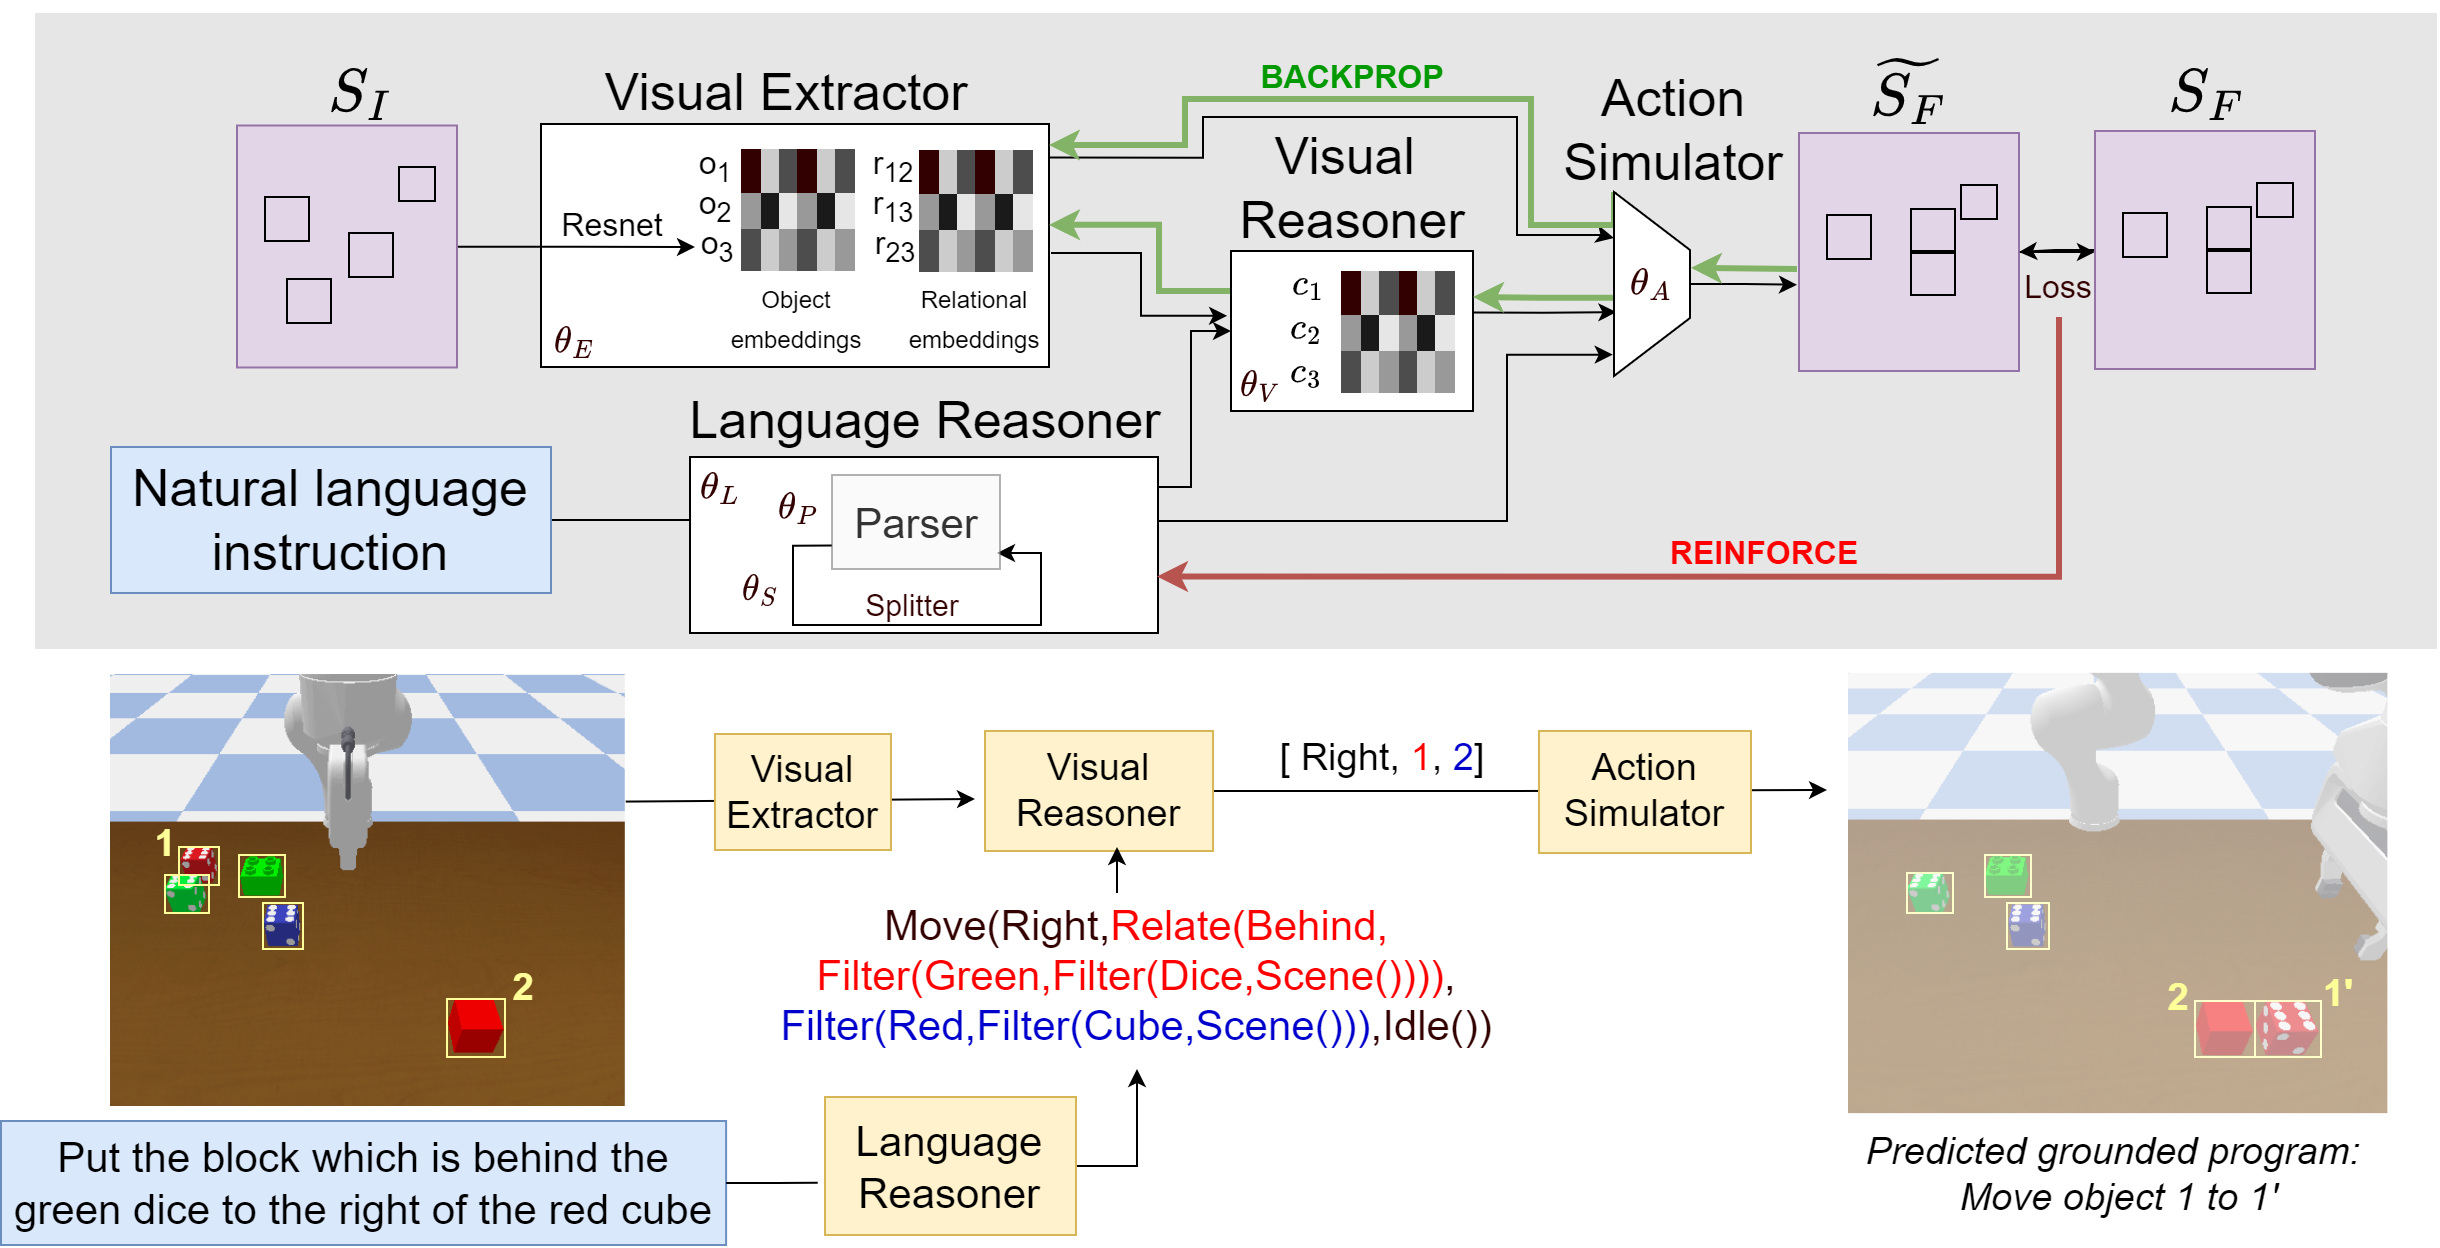
\includegraphics[width=\textwidth,clip,trim={0 20.5cm 0 0}]{figures/main-model-3.png}
    \caption{Neuro-symbolic Model architecture for learning manipulation programs}
    \label{fig:schematic}
\end{figure}

Unlike ~\cite{Mao2019NeuroSymbolic}, where the program execution is purely symbolic and deterministic, the program execution in our case is also neuro-symbolic. This brings difficulty in training the LR, but enables us learn the sub-goal generation. 
Finally, we also provide an encoder to extract objects from the initial scene $\tilde{S}_I$ , and a decoder to construct the final scene, $\tilde{S}_F$, once the sub-goals have been executed.


\begin{table}
    \centering
    \begin{tabular}{|p|p|p|p|}
    % \begin{tabular}{|p{0.01cm}|p{0.01cm}|p{0.08cm}|p{0.08cm}|}
        \hline
        \multicolumn{4}{|c|}{\textbf{Keywords and their classes}}\\
        \hline
         \multicolumn{2}{|c|}{\textbf{Object-level concepts}}& \multicolumn{2}{c|}{\textbf{Other concepts}} \\
         \multicolumn{2}{|l|}{\textbf{Color}: \{Red, Blue, Cyan,...\}}& \multicolumn{2}{l|}{\textbf{RelCpt}: \{Left, Behind, Front,...\}} \\
         \multicolumn{2}{|l|}{\textbf{Type}: \{Cube, Lego, Dice\}} & \multicolumn{2}{c|}{\textbf{ActCpt}:  \{MovRight, MovTop,...\}} \\
    \hline
    \hline
    \multicolumn{4}{|c|}{\textbf{Operators: ( Input $\rightarrow$ Output)}}\\
    \hline
    \multicolumn{2}{|l|}{Scene : None $\rightarrow$ ObjSet} & \multicolumn{2}{l|}{Unique: ObjSet $\rightarrow$ Obj}\\
     \multicolumn{2}{|l|}{Filter : (ObjSet, ObjCpt)$ \rightarrow$ ObjSet} & \multicolumn{2}{l|}{Relate  : (Obj, RelCpt) $\rightarrow$ ObjSet}\\
     \multicolumn{2}{|l|}{ Move : (ActCpt, World) $\rightarrow$ World} & \multicolumn{2}{l|}{ Idle :  World $\rightarrow$ World}\\
    \hline
    \multicolumn{4}{|c|}{ObjectSet $\in \mathbb{R}^{\text{N}}$, N = Num objects, Object = one-hot ObjectSet}\\
    \multicolumn{4}{|c|}{World = $\{(b_i,d)\}_{i=1}^\text{N} \in \mathbb{R}^5$, bounding boxes and depth for all objects }\\
    \hline
        \end{tabular}
    \caption{Domain Specific Language.}
    \label{table:dsl}
    \vspace{-0.5cm}
\end{table}

\begin{figure}
  \centering
  \begin{subfigure}{\textwidth}
      \centering
      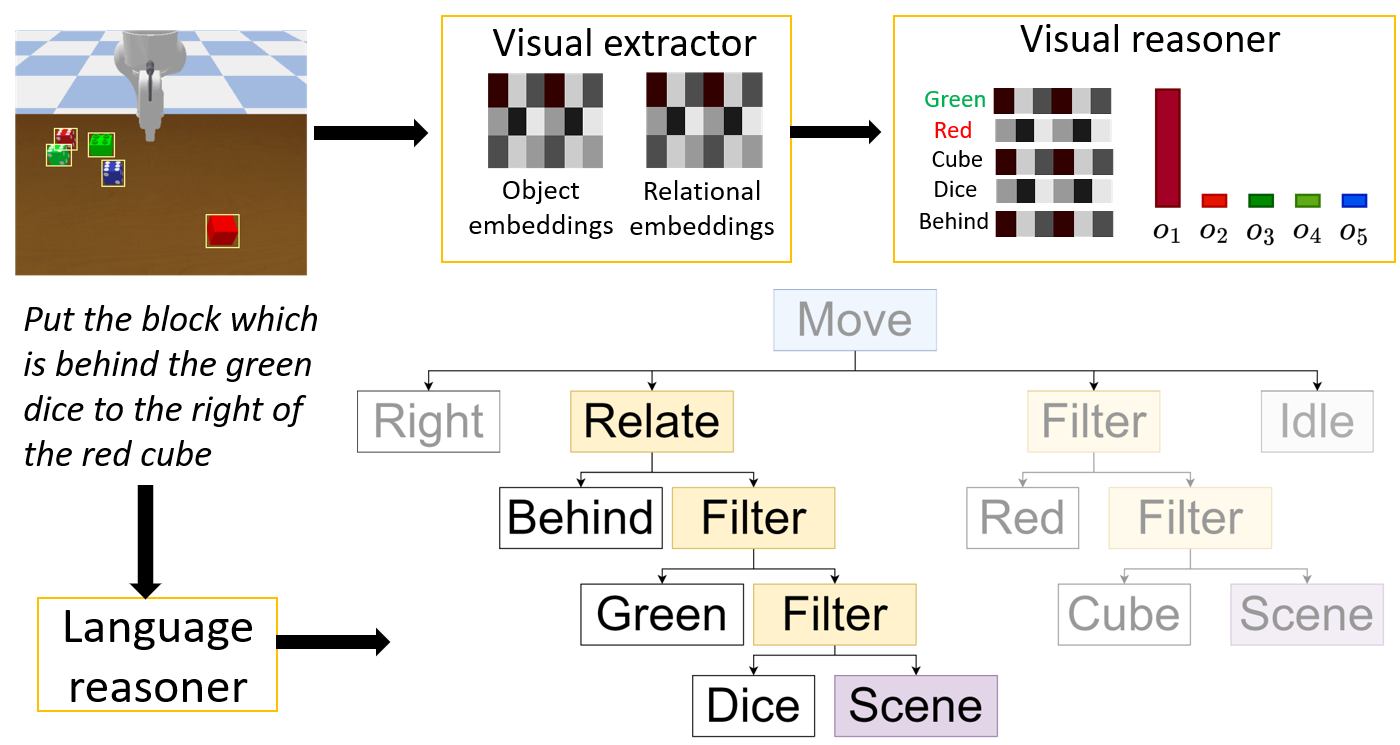
\includegraphics[width=\textwidth]{figures/example-1-n.png}
      \caption{Executing the emboldened sub-tree on the input scene}
      \label{fig:approach-1}
  \end{subfigure}

  \vspace{1cm}
  
  \begin{subfigure}{\textwidth}
      \centering
      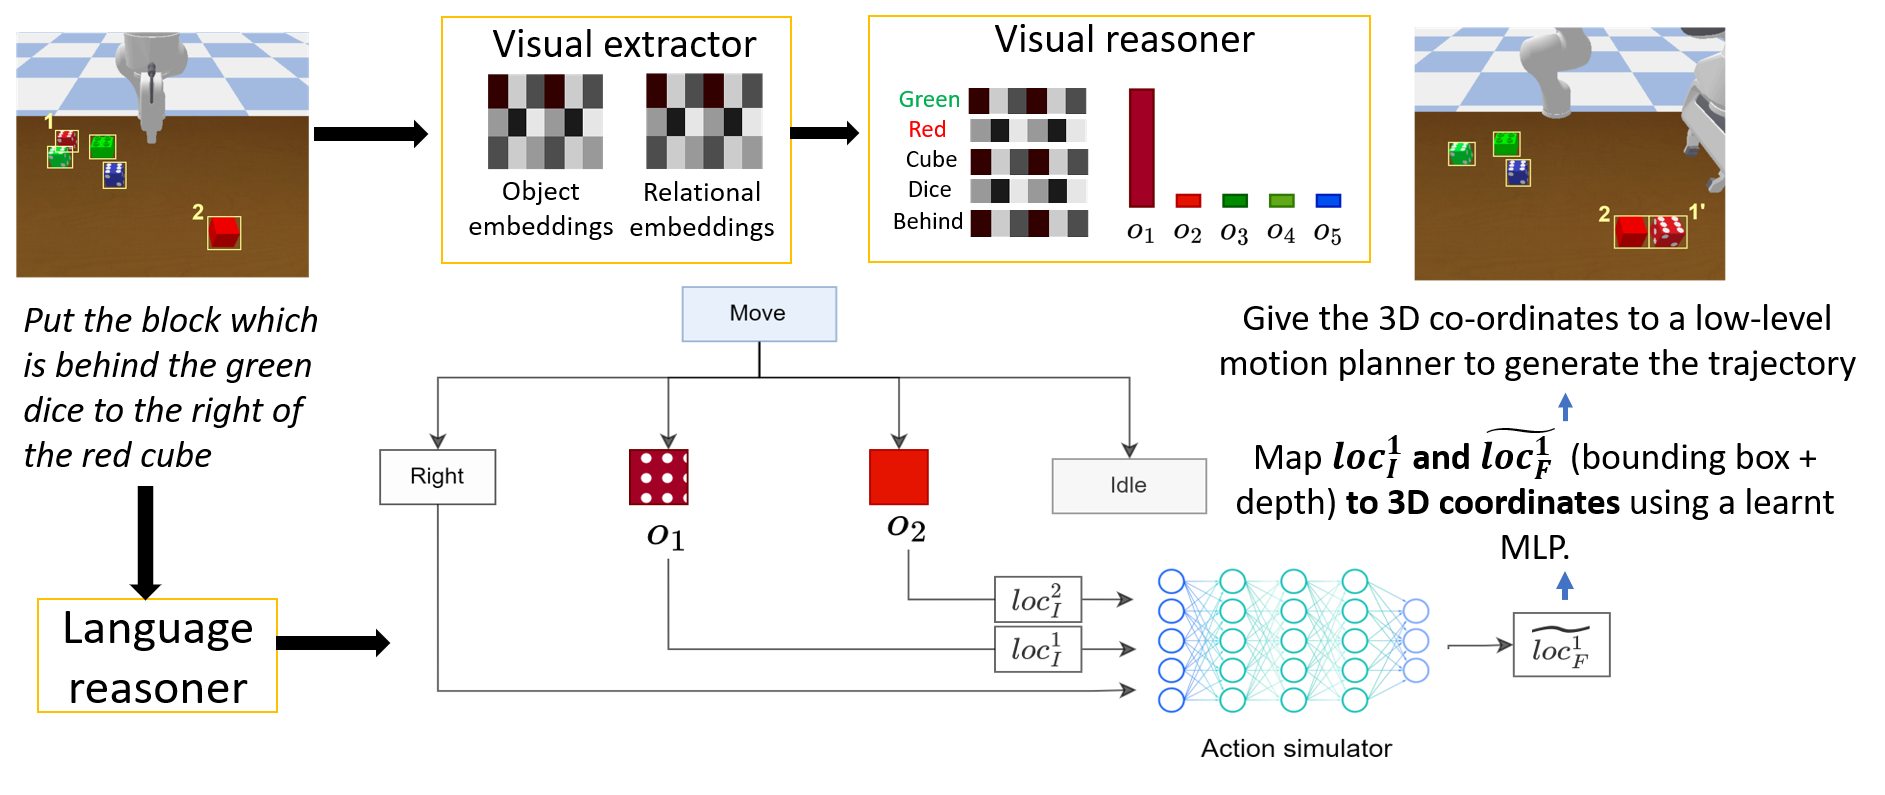
\includegraphics[width=\textwidth]{figures/example-2-n.png}
      \caption{VR computes the grounded program, which is used by the AS to compute the final location of the moved object, which is is fed into a low-level motion planner}
      \label{fig:approach-2}
  \end{subfigure}
  \caption{Quasi-symbolic program execution}
  \label{fig:approach}
\end{figure}

% Language Reasoner.
\subsection{Language Reasoner (LR)}
%
The language reasoner (LR) deduces a hierarchical symbolic program that corresponds to the 
manipulation task implied by the human's utterance to the robot. 
%
The deduced program consists of symbolic reasoning constructs that operate on neural concepts grounded in the state space of the scene and the action space of the robot. 
%
% Note that representation of a task as a hierarchical and compositional program facilitates deep reasoning over grounded concepts. 
%provided by symbolic constructs operating over grounded concepts. 
%
% Since a high-level task instruction may imply a sequence of actions, we adopt a hierarchical module where an LSTM~\cite{lstm} network first splits  the language instruction into a sequence of sub-instructions, each corresponding to one grounded action. The semantic parse of each sub-instruction is then inferred using a hierarchical  \emph{seq2tree} architecture similar to~\cite{dong2016language,Mao2019NeuroSymbolic}. The sequence of programs thus generated are composed to produce the symbolic program for the original language instruction.
% 
Since a high-level task instruction may imply a sequence of actions, we adopt a hierarchical model where an LSTM~\cite{lstm} network first splits the instruction into a sequence of sub-instructions, each corresponding to one grounded action. The semantic parse of each sub-instruction is then inferred using a hierarchical  \emph{seq2tree} architecture similar to~\cite{dong2016language,Mao2019NeuroSymbolic}. The sequence of programs thus generated are composed to produce the symbolic program for the original language instruction.
%
%
% Overall the LR module resembles a \emph{seq2tree} architecture that builds on ~\cite{dong2016language,Mao2019NeuroSymbolic} 
%
%The language reasoner (LR) has two parts (i) a splitter that breaks a multi-step instruction into a sequence of single step instructions, and (ii) a semantic parser, similar to ~\cite{dong2016language} and ~\cite{Mao2019NeuroSymbolic}, which takes each single step instruction and outputs a hierarchical program.  
%
%Formally, assuming a bound, $L_{max}$, on the word tokens representing a single step execution, 
%an arbitrary instruction $\Lambda = \lambda_{0:n} \coloneqq \{\lambda_0, \lambda_1,\cdots,\lambda_n\}$, at every step $t$, the splitter first decides a part of the sentence $\lambda_{0:l_t} \subset \lambda_{0:L_{max}}$ to be processed. The parser then takes $\lambda_{0:l_t}$ and  outputs a program $p_t$. The processed sub-string $\lambda_{0:l_t}$ gets removed and the process continues with the remaining part $\lambda_{l_{t}+1:n}$ of the instruction.
%Finally, the programs $p_1,\cdots p_T$ are composed into a single program $\mathtt{P}$, which will be used by the Visual Reasoner for grounding and execution. 


%For predicting the break point $l_t$, at the step $t$, the splitter encodes the first $L_{max}$ tokens it encounters using an LSTM [64] and outputs the hidden state, $h_t$ for each token. Then, a fully connected layer followed by a soft max layer outputs a probability distribution over the tokens for choosing a potential break point. The architecture of the semantic parser is very similar to that of the seq-to-tree parser (with slight changes in the kind of attention used) proposed by ~\cite{dong2016language} and later used by ~\cite{Mao2019NeuroSymbolic}; we refer to prior work for details.
%; we make use of additional attention with few extra attention to deal the action concepts. 

% VE Module
\subsection{Visual Extractor (VE)}
\label{subsec:visual-reason}
The visual extractor forms an object-centric view of the world by extracting object proposals in the form of bounding boxes for the objects using a pre-trained object detector~\cite{redmon2016you}. 
%
Following~\cite{Mao2019NeuroSymbolic}, dense object representations are obtained by passing the bounding boxes (after non-maximal suppression) through a feature extractor as~\cite{targ2016resnet}. 
The data association between object proposals in initial/final scenes is estimated greedily based on cosine similarity between the dense object features in both scenes.

% Visual Reasoner
\subsection{Visual Reasoner (VR)}
%
The visual reasoner performs visuo-spatial, object-centric reasoning to compute a sequence of sub-goals grounded in the scene from the symbolic program.
%
E.g., the instruction \textit{``put the block which is behind the green dice"} requires the robot to perform reasoning to resolve the specific world object that conforms to the relations/attributes as being behind a dice with colour attribute of green. 

The visual reasoner parameterizes object-level and relational concepts in the DSL (Table ~\ref{table:dsl}) with neural embeddings. Similar to ~\cite{Mao2019NeuroSymbolic}, a differentiable framework is defined for the execution of operators such as \emph{Filter, Unique, Relate, Idle}.  \\ 
%
As in ~\cite{Mao2019NeuroSymbolic}, intermediate results of execution are represented in a probabilistic manner. For e.g., a set of objects is represented as a vector of probabilities where the $i$-th element represents the probability of the $i$-th object being an element of the set. \emph{Filter, Unique, Relate} etc. sequentially modify this vector to ultimately yield the referred object/set of objects.  \\ 
%
This execution framework is used to execute the symbolic program  on top of the visual features (extracted by the visual extractor) resulting in the grounding of the program, $\Pi$, on the world state.


% Action simulator
\subsection{Action Simulator (AS)}
\label{subsec:action-simulator}
The action simulator learns the semantics of action concepts of the DSL. It takes as input, the action concept, the initial locations  of the object to be manipulated and the reference object respectively and outputs the target location of the former. The outputted target location of the object being manipulated serves as a sub-goal for the low-level motion planner. We determine the location of an object by the corners $b = (x_1,y_1,x_2,y_2)$ of the enclosing bounding box and the depth of the object from the camera face. 

\noindent  
Overall, the model can be summarized as follows:
\begin{itemize}
    \item $\mathtt{P} \leftarrow \mathtt{LR}(\Lambda; \theta_P, \theta_S)$, where $\mathtt{P}$ is a symbolic program composed of DSL constructs. 
    \item $\Pi \leftarrow \mathtt{VR}(\mathtt{P}, \mathtt{VE}(S_I;\theta_E);\theta_V)$. The visual reasoner then grounds $\texttt{P}$ and outputs $\Pi$, the grounded program. For example, in Figure \ref{fig:schematic}, red and blue subprograms are grounded to object 1 and 2 respectively.
    \item $G \leftarrow \text{AS}(\Pi; \theta_A)$. The action simulator then takes $\Pi$ and returns a sequence of sub-goals, $G = (g_0, g_1, ..., g_{n-1})$, for the motion planner.
\end{itemize}
Here, $\theta$'s are the parameters of the corresponding  module. 

\subsection{Loss Function and Model Training}
\label{subsec:loss&training}
%Model training optimizes the following loss:
%Let $\Theta$ = ($\theta_E$, $\theta_S$, $\theta_P$, $\theta_V$, $\theta_A$) be the parameters of the visual extractor, splitter, parser, visual reasoner and the action simulator respectively. Given instruction $\Lambda$ and initial scene $S_I$, 
% \\[-1cm]
% \begin{align*}
% \begin{split}
%      \mathtt{P} \leftarrow LR(\Lambda ; \theta_P, \theta_S) \\ 
%      \widetilde{S}_F & \leftarrow ManipulationProgram(S_I, \Lambda)\\[-0.1cm]
%      & \resizebox{0.9\hsize}{!}{ $=  AS\Big(VR\big( LR$(\Lambda ; \theta_P, \theta_S), VE(S_I ; \theta_E) ; \theta_V\big) ,LR(\Lambda ; \theta_P, \theta_S); \theta_A} \Big)\\
% \end{split}
% \end{align*}
% \\[-1cm]
%\begin{align*}
%    \resizebox{\hsize}{!}{\widehat{\Theta} \leftarrow \text{argmax}\limits_{\Theta} \;\mathbb{E}_\mathtt{P}\Big[\text{IoU}\big(S_F, Simulate(\mathtt{P} = ManiProg(S_I, \Lambda; \Theta))\big) \Big]}
%\end{align*}
%\textbf{Training on single-step instructions}. 
Given a single-step instruction $\Lambda$, the parser predicts a symbolic program $\mathtt{P}$. The visual reasoner grounds $\mathtt{P}$ to predict a sequence of sub-goals. The action simulator computes the low-level action corresponding to each sub-goal. The sequence of low-level actions is executed on the initial scene $S_I$ to get the predicted final locations of the objects $\{\widetilde{loc}^i_F\}_{i=1}^N$. Let $\{{loc}^i_F\}_{i=1}^N$ be the true locations in the gold final state, $S_F$. As mentioned above $loc = (b,d)$, where $b$ is the corners of bounding box and $d$ is the depth. The loss function $L_{act}\coloneqq \sum_i^N\|\widetilde{loc}^i_F- loc^i_F\|
+ \beta (1-\text{IoU}(\widetilde{b}^i_F, b^i_F))$ is used to train the action simulator and the visual modules. 
Since there is no explicit supervision to the parser, we train the parser using the policy gradient algorithm REINFORCE with the reward set to $-L_{act}$. 
%
During initial training, an explicit expectation (subtracting the mean action loss as the baseline) is computed over all programs to inform the loss, ameliorating the variance issue arising in REINFORCE.
%
The Language Reasoner is trained using REINFORCE and the other modules using backpropagation.
%
%expectation over $\mathbb{E}_{\mathcal{P}}[-L_{act}(P)]$ over the program space $\mathcal{P}$ and use this as reward to the parser.
%
 %The parameters $\theta_E$, $\theta_V$ and $\theta_A$ are trained by back propagation from the expected action loss, $\mathbb{E}_{\mathcal{P}}[L_{act}(\mathtt{P})]$, and $\theta_P$ is trained by REINFORCE using $\mathbb{E}_{\mathcal{P}}\big[\sum_{\mathtt{P}\in \mathcal{P}}{L_{act}(\mathtt{P})} + L_{par}(\mathtt{P})\big$]. 
%
\iffalse
Once we have trained the other modules on single step commands, we train the splitter on all one and two step commands in the training set. The splitter computes the probability $\mathcal{S}(s;\theta_s)$ of breaking the sentence on each token $s$ of the first $L_{max}$ tokens. The training objective, for a sentence $\Lambda$, can be described as 
\[
    \resizebox{\hsize}{!}{\[\theta_S \leftarrow \text{argmin} \Big( \mathbb{E}_{s\sim{\mathcal{S}}}\big[L_{act}(Compose(Parser(L_{0:s}),Parser(L_{s+1:}))\big]\Big)\]}
\]
 where $Compose$ takes input symbolic programs generated by the parser for single step instructions and composes them hierarchically. Since all other modules are already trained for single step sentences. The splitter learns to split the large sentences at the correct positions. 
 \fi
% We do not have direct access to the true plan $G$. We also do not have access to intermediate object locations. The only information we have is the locations of the objects in the  the final scene $S_F$.   Let $loc_i \equiv (b_i, d_i)$ denote the true location (in the image space) of object $i$, in the final scene $S_{T+1}$. Recall that $b_i, d_i$ are bounding box and mean depth of the object $i$ respectively. Let $\widehat{loc}_i$ denote the final location of object $i$ as predicted by our model. Then, we compute the loss (for object $i$) $\mathcal{L}(\widehat{loc_i},loc_i)$ as a combination of two terms, $w_1 * {\tt MSE}(\widehat{loc_i},  loc_i) +w_2 * (1- {\tt IoU}(\widehat{b_i}, b_i))$. The first term is the mean squared error between true and predicted locations, and the second term is one minus intersubsection over union (IoU) between the true and predicted bounding boxes. $w_1,w_2$ are hyper-parameters determining the important of two loss terms, and are set using a validation set. The total loss, $L$, is simply average of the loss over each object, i.e., $\sum_{i=1}^{N} \mathcal{L}(\widehat{loc_i}, loc_i)/N$. The reward signal passed to the parser is computed as, $R  = R_0 - L$ where $R_0$ is a hyper-parameter.

The following training curriculum is adopted: (i) training on single step commands with reasoning involving individual object features only, 
(ii) the trained action simulator module is frozen and additional training on single step commands involving reasoning over spatial relations between objects is carried out. 
(iii) the sentence splitter in the Language Reasoner module is fine-tuned on multiple-step instructions. 

\subsection{Scene Reconstruction}
We additionally train a neural model to synthesize the scene corresponding to each sub-goal, given only the initial scene and predicted object locations. This enables us to visualise the scene modification without the need of execution by a robot manipulator along with providing interpretability to the model's latent program space. Our approach is adapted from \cite{dhamo2020_SIMSG}.

\begin{figure}
    \centering
    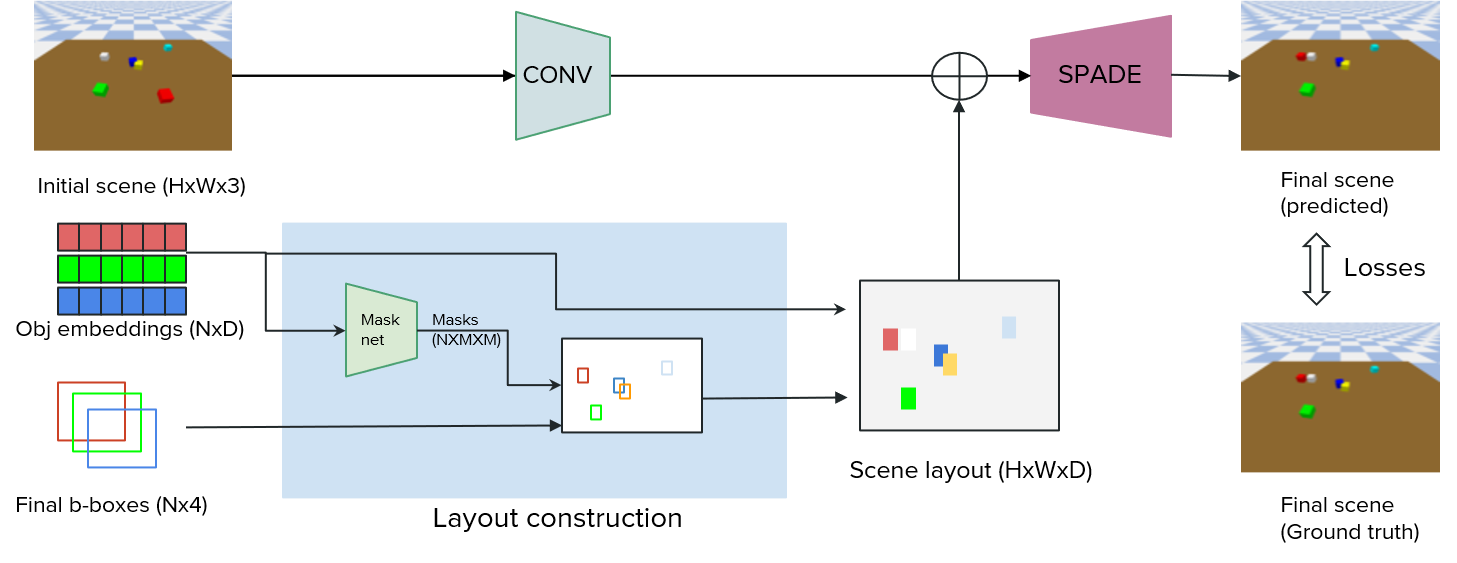
\includegraphics[width=\textwidth]{assets/recons-arch.png}
    \caption{Scene reconstruction architecture}
    \label{fig:recons}
\end{figure}

The reconstruction architecture can be seen in figure \ref{fig:recons}. The scene graph is constructed with nodes having object embeddings (N objects, each with an embedding of size D) and bounding boxes (N objects, each with a bounding box of size 4). This graph is updated with predicted bounding boxes corresponding to final locations of the objects after any given step. A scene layout is created by stacking the object features according to their corresponding final locations. This layout is concatenated with the initial image features, and passed through the SPADE decoder. The final scene is used for supervison, with a weighted sum of the several pixelwise and discriminator-based losses, similar to \cite{dhamo2020_SIMSG}. This trained model can now be used to reconstruct any intermediate scene, by updating the predicted bounding boxes in the scene graph corresponding to the subgoals at each step, as shown in figure \ref{fig:recons-steps}

\begin{figure}
    \centering
    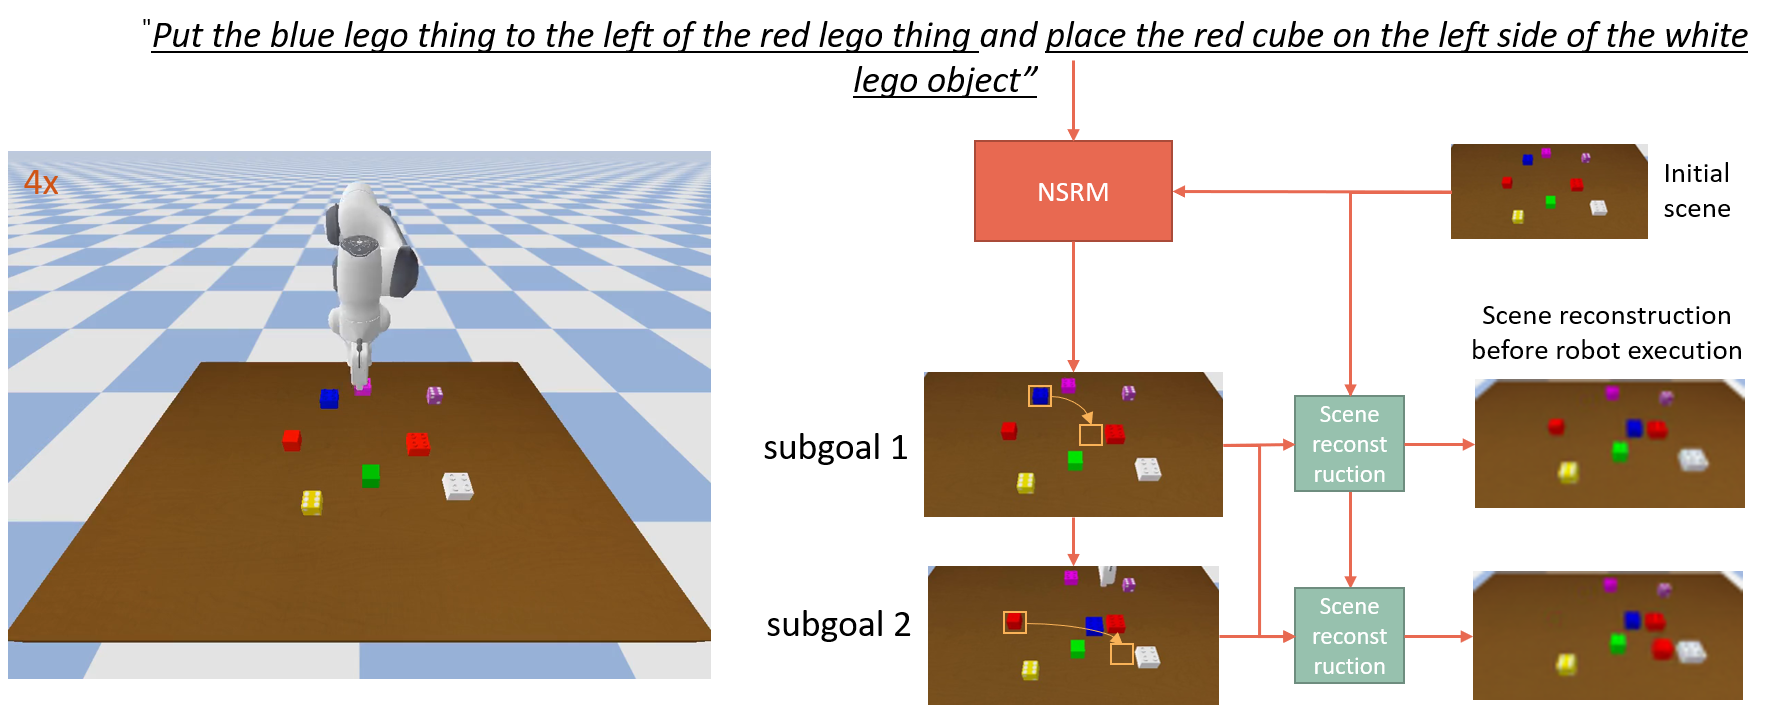
\includegraphics[width=\textwidth]{assets/recons-steps.png}
    \caption{Scene reconstruction at each step before the actual execution}
    \label{fig:recons-steps}
\end{figure}

